\documentclass[12pt]{report}
\usepackage{amssymb}
\usepackage{multicol}
\usepackage{graphicx}
\usepackage{subfigure}
\usepackage{verbatim}
\usepackage[letterpaper,left=1cm,right=2cm, top=1.5cm,
bottom=1.5cm,head=0cm,foot=1cm]{geometry}

\parindent=0in

\newcommand{ \probDir}[1]{{ \bf\small #1 \mbox{  }}}

\newcommand{ \breakList}{\setcounter{saveenum}{\value{enumi}} \end{enumerate}}
\newcommand{ \contList}{\begin{enumerate} \setcounter{enumi}{\value{saveenum}}}

\newcounter{saveenum}

\def \wspace{4cm}

%%%%%%%%%%%%%%%%%%%%%%%%%%%%%%%%%%%%%%%%%
\begin{document}

{\bf{Honors Physics} \hfill {Quiz 1: Math Skills} \hfill {Mr. Kelley}} \\ \\
%%%%%%%%%%
\probDir{Solve the following equations for $x$, and simplify:} \\
%%%%%%%%%%
\begin{multicols}{2}
\begin{enumerate}
\item $\frac{9}{8x} =  3z$
\vspace{\wspace}
\item $6z - 2zx = 12zy$
\vspace{\wspace}
\item $F=k\frac{ab}{x^2}$
\vspace{\wspace}
\item $8tx + 8t = 12x$
\vspace{\wspace}
\breakList
\end{multicols}

\vspace{\wspace}

%%%%%%%%%%
\probDir{Write $x$ as a function of $t$, and simplify:}
%%%%%%%%%%
\begin{multicols}{2}
\contList
\item $6t + 3x = 9$
\vspace{\wspace}
\item $t^2 - 2xt = t$
\vspace{\wspace}
\item $8xt = 6t^2 +2x - 10t$
\vspace{\wspace}
\item $\frac{x}{t} - v_{\circ}= \frac{1}{2}at$
\breakList
\end{multicols}
\vspace{\wspace}
\pagebreak
\contList

\item \probDir{What is the value of $x(3)$ in the following figures?}
\begin{figure}[h]
\centering
\subfigure[]{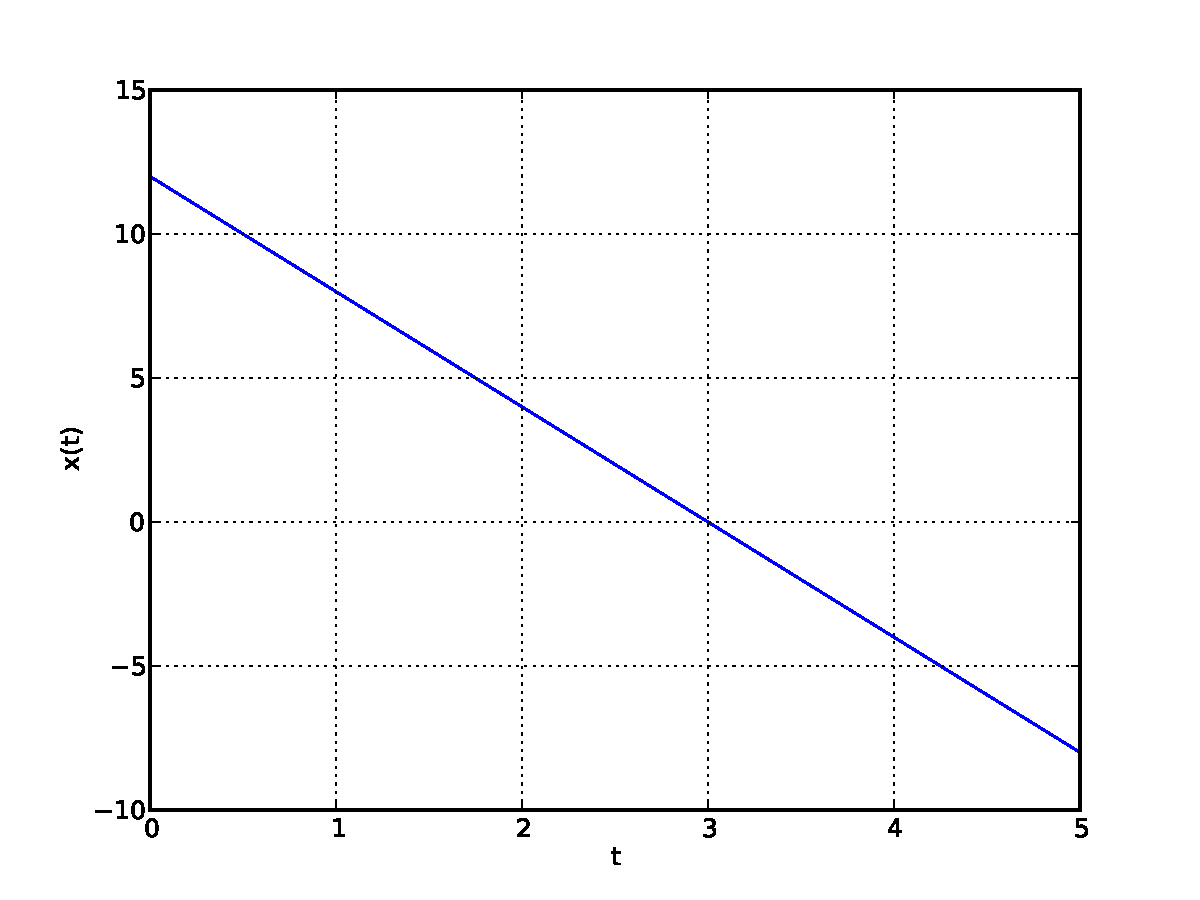
\includegraphics[scale = .45]{fig1.pdf}}
\subfigure[]{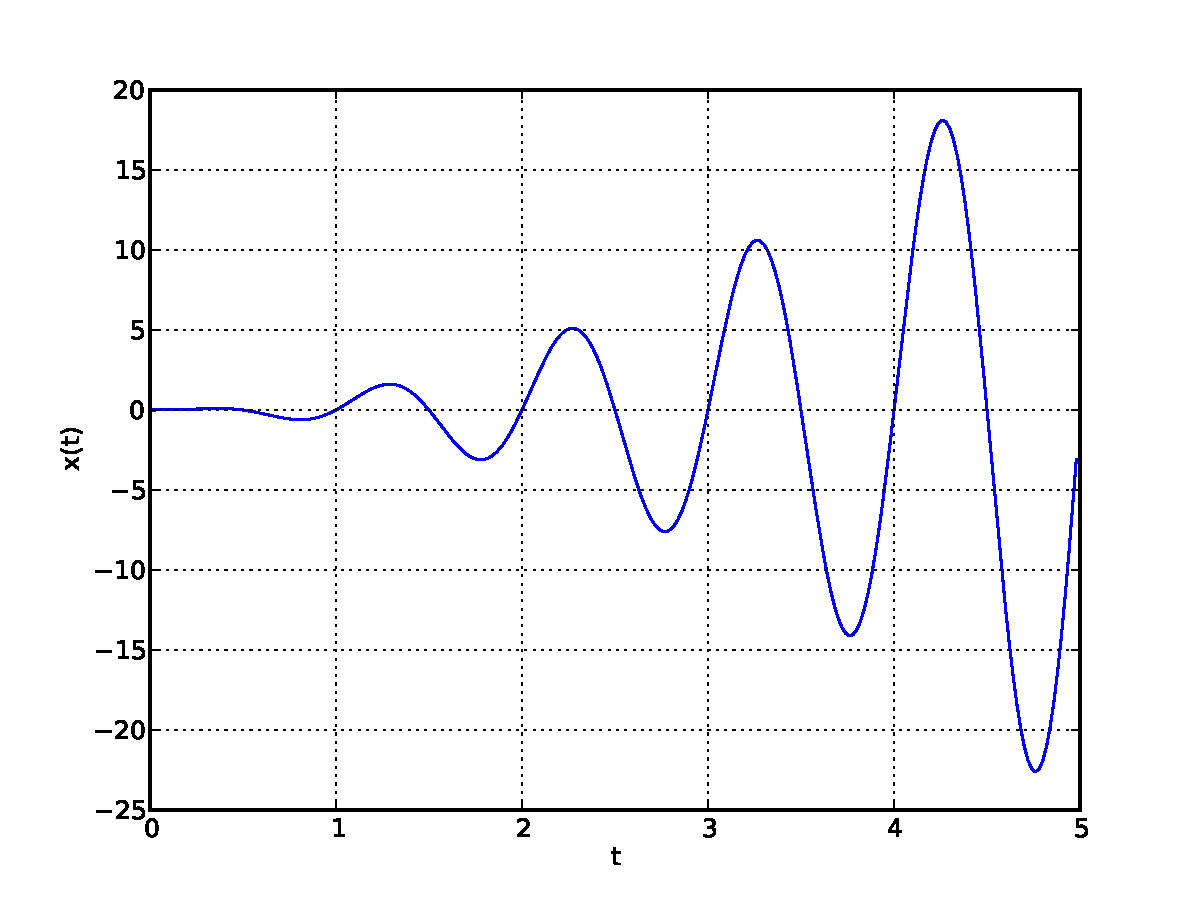
\includegraphics[scale = .45]{fig2.pdf}}
\setcounter{subfigure}{0}
\end{figure}

\item \probDir{What is the value of $x(4)$ in the following figures?}
\begin{figure}[h]
\centering
\subfigure[]{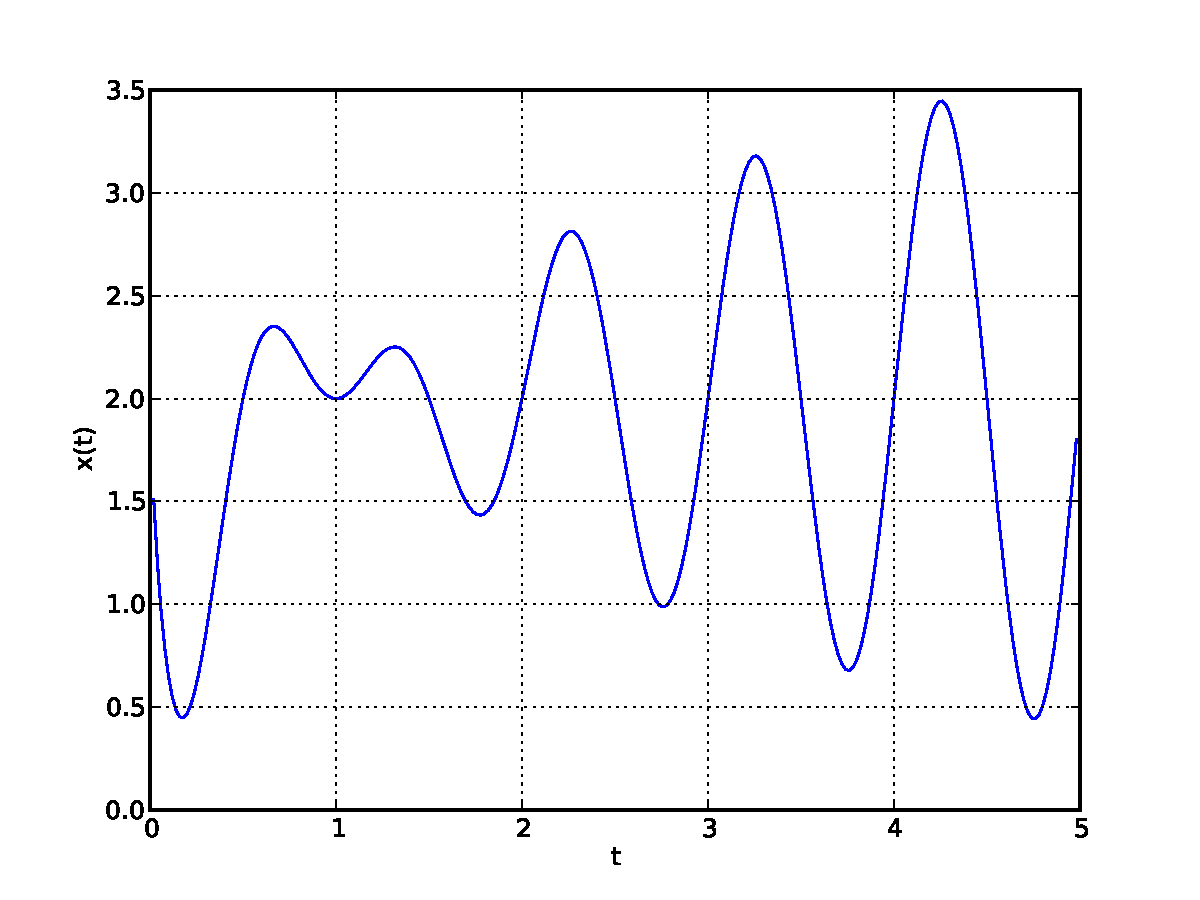
\includegraphics[scale = .45]{fig22.pdf}}
\subfigure[]{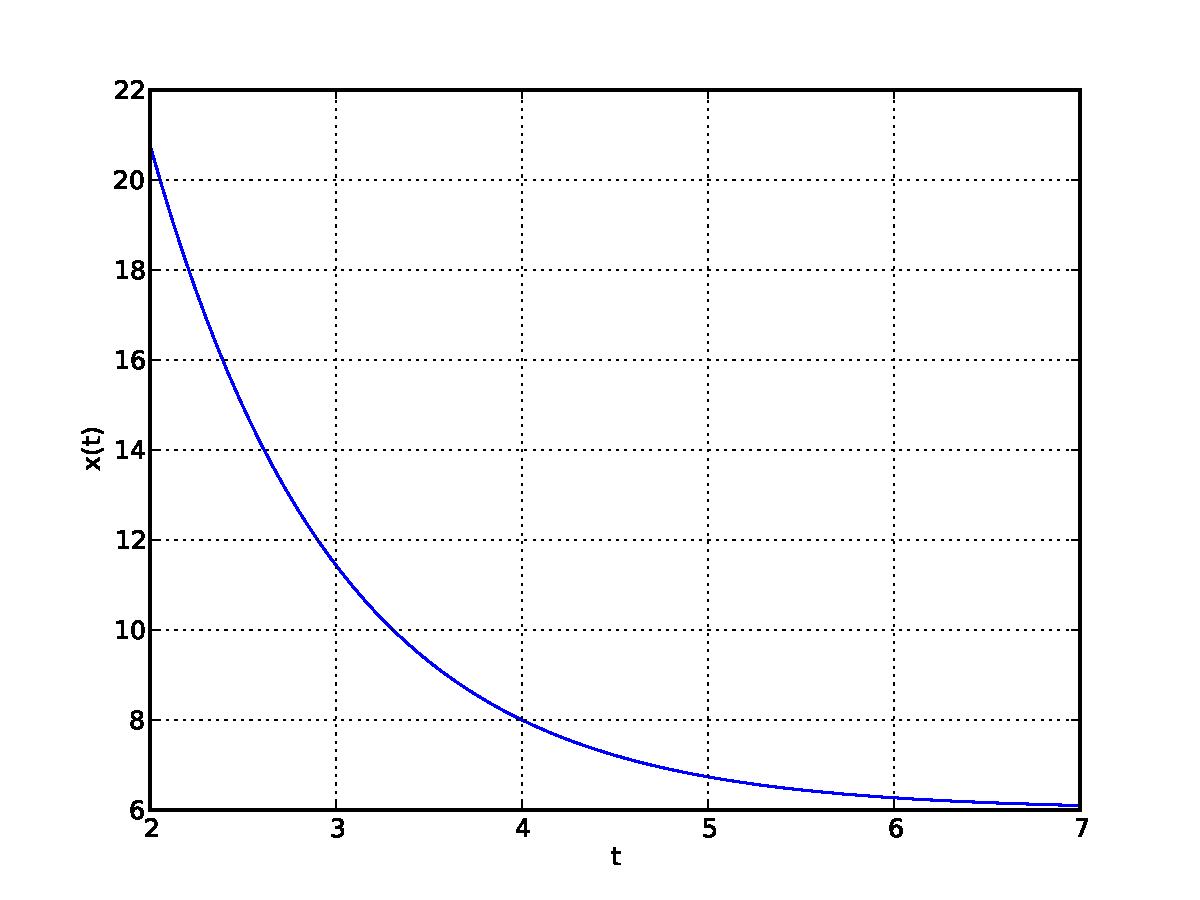
\includegraphics[scale = .45]{fig23.pdf}}
\setcounter{subfigure}{0}
\end{figure}


%%%%%%%%%%%%%%

\item What is $x(\frac{1}{2})$ in problem 7?
\vspace{2cm}
\item What is $x(2)$ in problem 10?

\pagebreak

\item \probDir{Find $a$ and $b$ in the following figures.}

\begin{figure}[h]
\centering
\subfigure[]{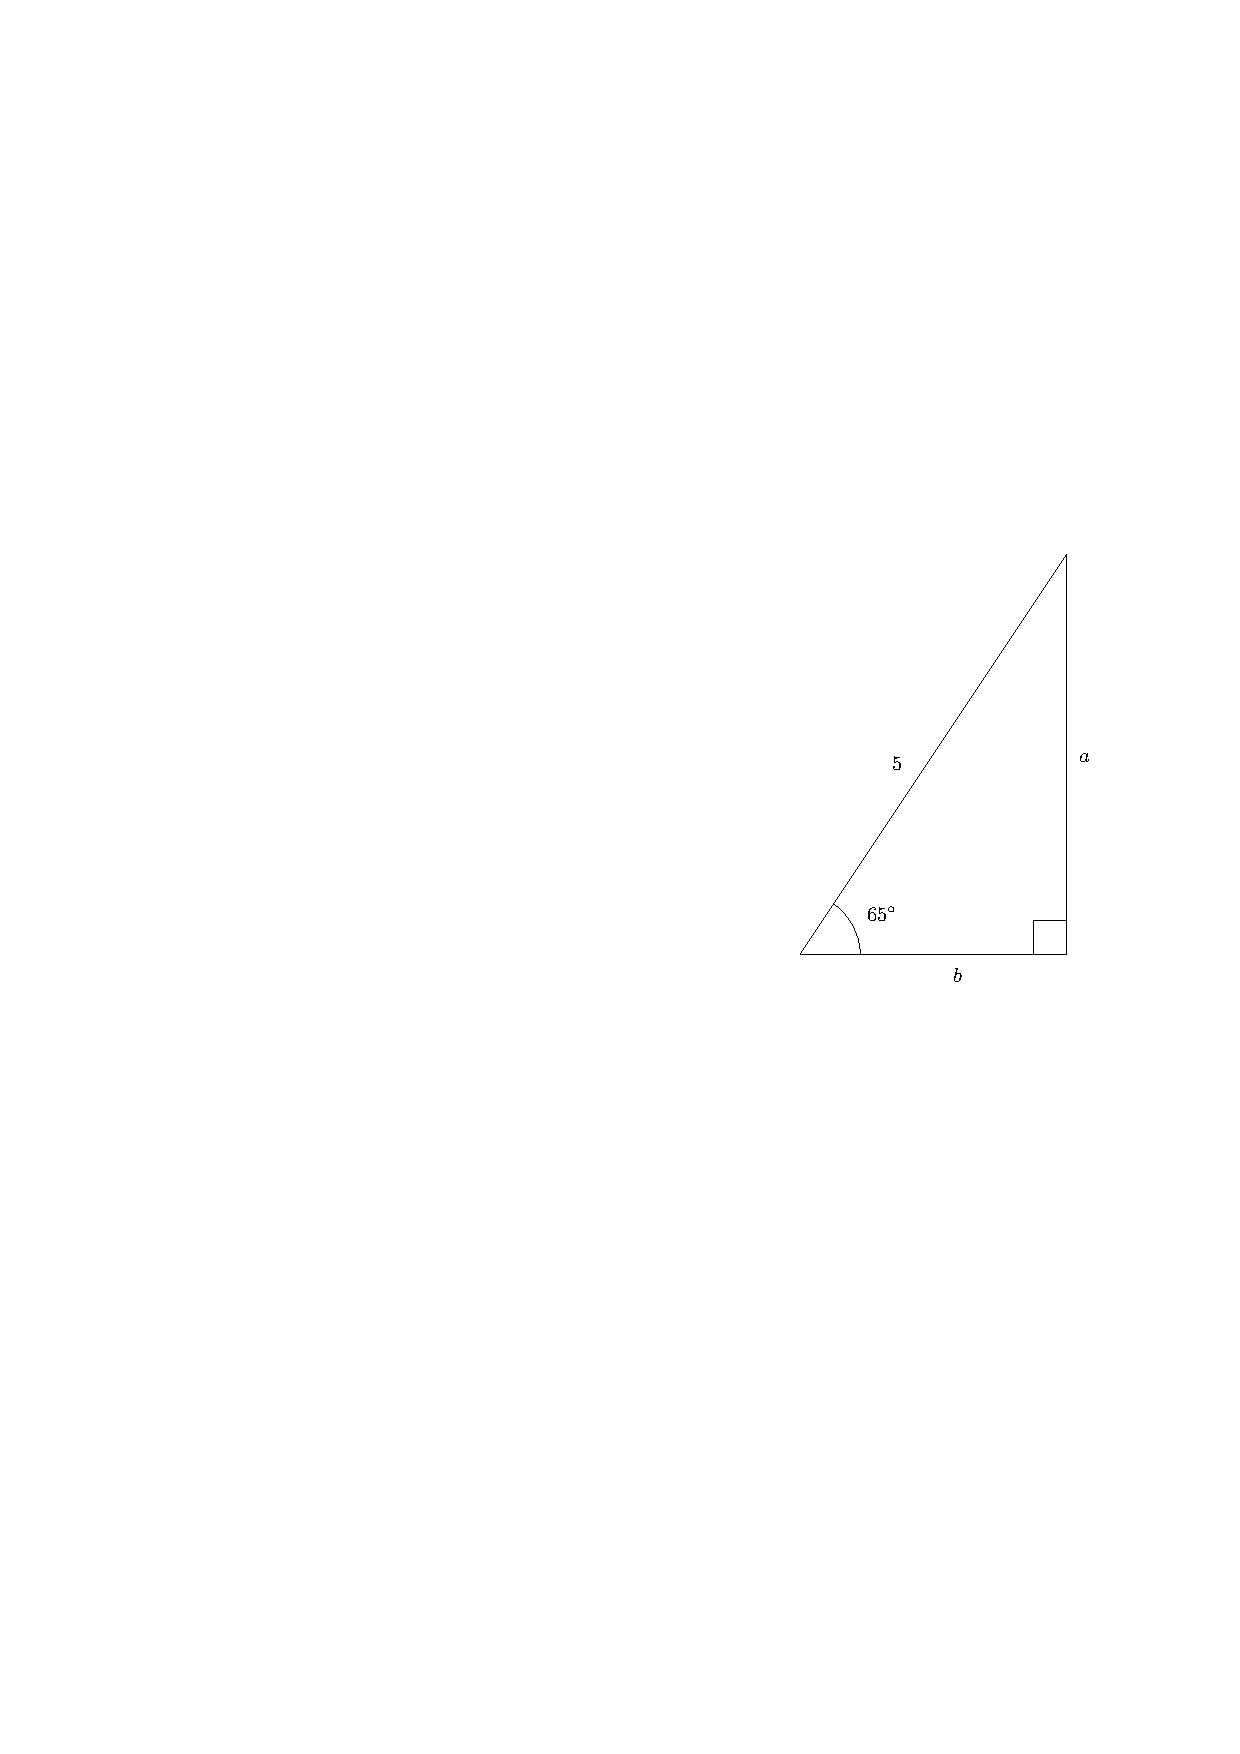
\includegraphics[scale = .8]{rt3.pdf}} \hspace{3cm}
\subfigure[]{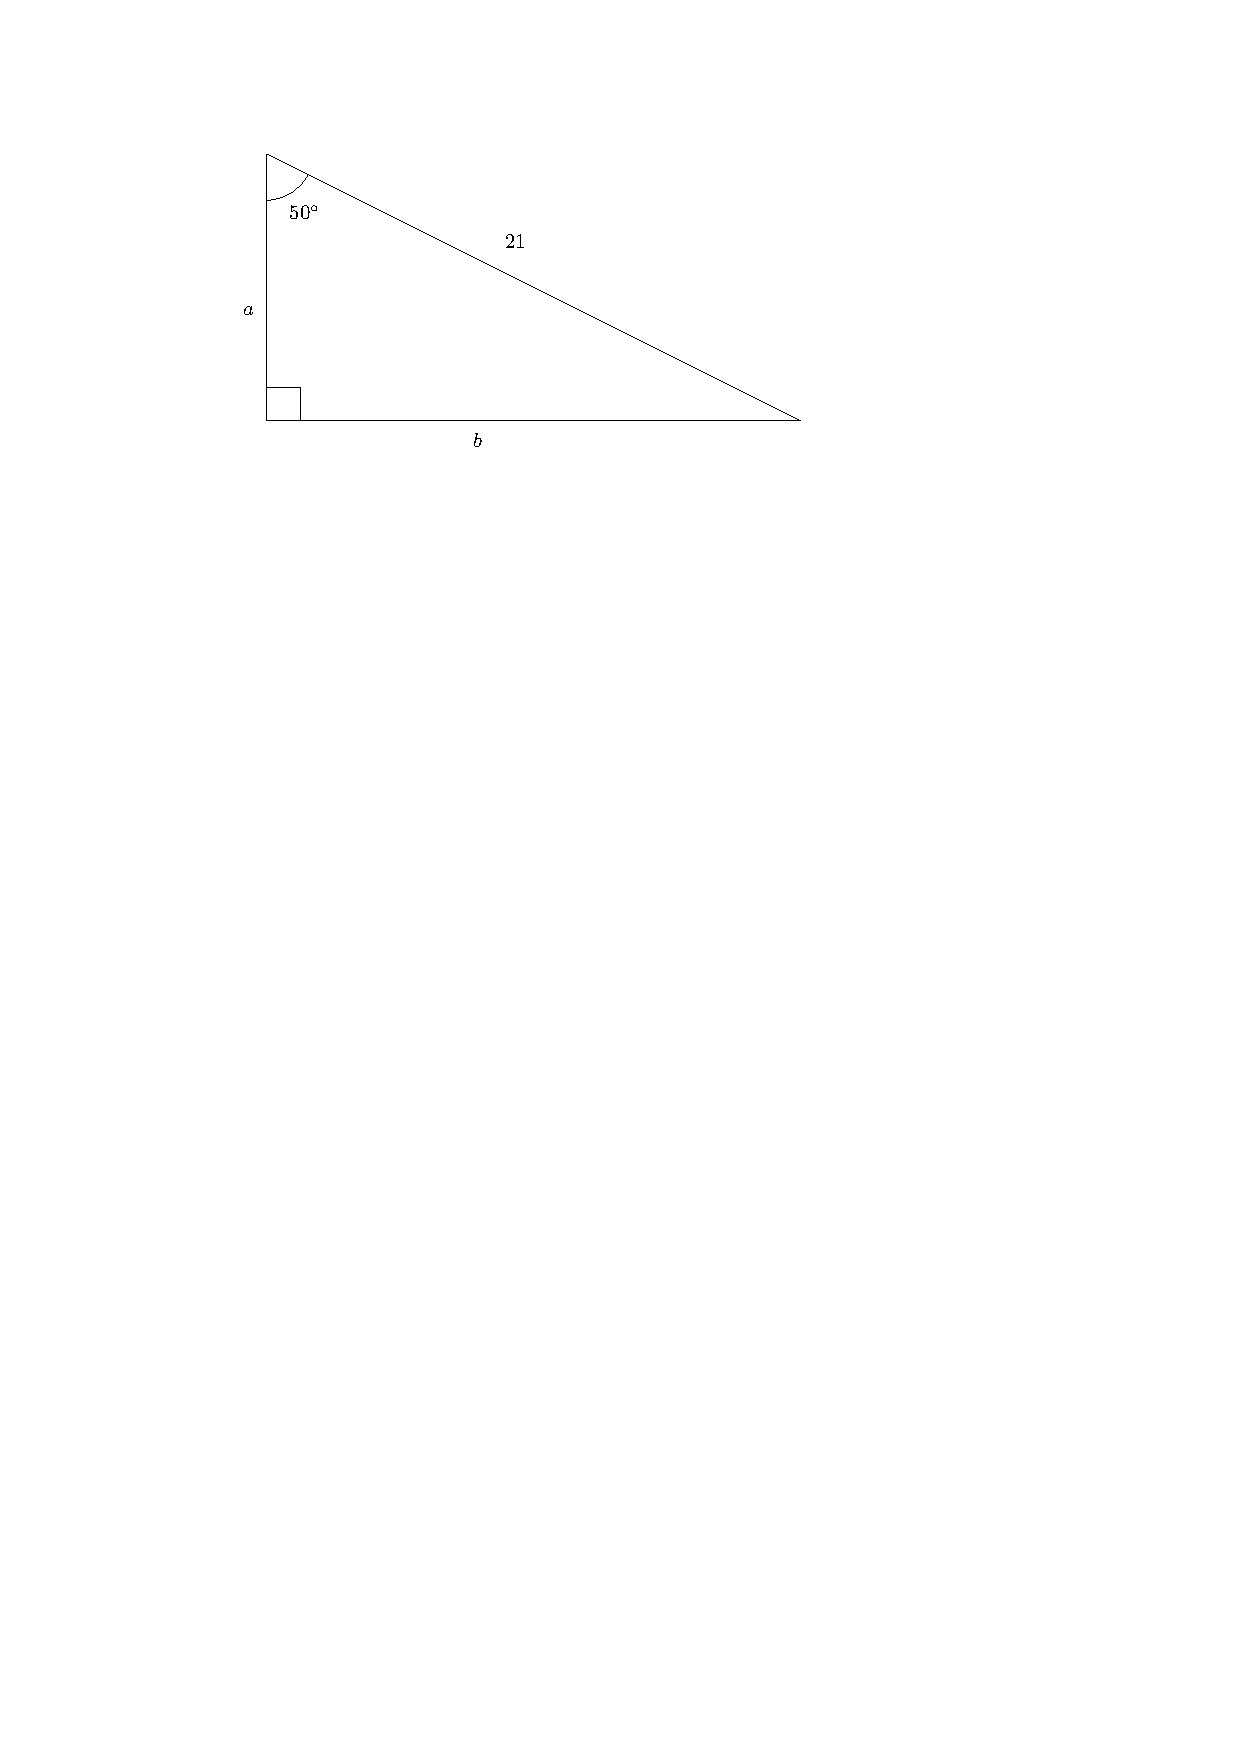
\includegraphics[scale = .8]{rt1.pdf}}
\setcounter{subfigure}{0}
\end{figure}
\vspace{\wspace}
\vspace{\wspace}

\item Convert $1.08 \times 10^{9} \mbox{ km/h}$ to units of m/s.



\end{enumerate}

\end{document}